%By conference call, March 7, 2018 and onward
\documentclass[11pt,compress,xcolor={usenames,dvipsnames},aspectratio=169]{beamer}
%slides and notes
%\usepackage{amsmath,datetime,xmpmulti,mathtools,bbm,array,booktabs,alltt,xspace,mathabx,pifont,tikz,calc,colortbl,stmaryrd,graphicx}
\usepackage{amsmath,datetime,xmpmulti,
	mathtools,
	bbm,
%	mathabx,
	array,
	relsize,
	booktabs,alltt,xspace,tikz,calc,colortbl,graphicx}
\usepackage[usenames]{xcolor}
\usepackage[tikz]{mdframed}
%\usepackage[author-year]{amsrefs}
\usepackage[style=nature]{biblatex}
\addbibresource{FJHown23.bib}
\addbibresource{FJH23.bib}
\usepackage{newpxtext}
\usepackage[euler-digits,euler-hat-accent]{eulervm}
%\usetikzlibrary{arrows}
\usepackage{cleveref}
\usepackage{algorithmic}
\usepackage{media9}

\usetheme{FJHSlimNoFoot169}

\definecolor{ltred}{rgb}{1,0.75,0.75}

\addtolength{\FJHCovImageVOffset}{-5ex}

\setlength{\parskip}{2ex}
\setlength{\arraycolsep}{0.5ex}

% from mathabx.sty and mathabx.dcl
\DeclareFontFamily{U}{mathx}{\hyphenchar\font45}
\DeclareFontShape{U}{mathx}{m}{n}{
	<5> <6> <7> <8> <9> <10>
	<10.95> <12> <14.4> <17.28> <20.74> <24.88>
	mathx10
}{}
\DeclareSymbolFont{mathx}{U}{mathx}{m}{n}
\DeclareFontSubstitution{U}{mathx}{m}{n}
\DeclareMathAccent{\widebar}{0}{mathx}{"73}

\newcommand{\insertitemmarker}{\alert{\leavevmode\usebeamertemplate{itemize item}} \ }

%\makeatletter
%\newcommand{\vast}{\bBigg@{3}}
%%\newcommand{\vast}{\bBigg@{4}}
%\newcommand{\Vast}{\bBigg@{5}}
%\makeatother


\mdfdefinestyle{redshade}{%
	leftmargin=0 pt,
	rightmargin = 0pt,
	innerleftmargin = 1ex,
	innerrightmargin = 1ex,
	skipabove = 0 pt,
	skipbelow = 0 pt,
	backgroundcolor=red!20,
	linecolor=red!20,
	roundcorner=5pt}

\title[]{Function Approximation When Function Values Are Expensive}
\author[]{Fred J. Hickernell\inst{1} \and Simon Mak\inst{2} \vspace{2ex}}
\institute{\inst{1} Department of Applied Mathematics, Illinois Institute of Technology, \href{mailto:hickernell@iit.edu}{\url{hickernell@iit.edu}}  \and
	\inst{2} School of Industrial and System Engineering,  Georgia Institute of Technology}
\thanksnote{
	Supported by NSF-DMS-1522687 and DMS-1638521 (SAMSI)}
\event{SAMSI-QMC Transition Workshop}
\date[]{May 7, 2018}

%Title:  Guaranteed Fixed-Width Confidence Intervals for Monte Carlo and Quasi-Monte Carlo Simulation

%Abstract: When performing a simulation to determine $\mu=\mathbb{E}(Y)$ one wonders what the error is and how many samples are required to achieve a desired accuracy.  We may want a confidence interval for the of the form $\mathbb{P}[\lvert\mu - \hat{\mu}_n\rvert\le \varepsilon] \ge 99\%$ where $\varepsilon$ is fixed by the user, and the number of samples, $n$, must be determined to make the sample mean, $\hat{\mu}_n$ close enough to the true mean.  Popular confidence intervals are based on large sample results, such as the Central Limit Theorem, or heuristics, but these error estimates can be fooled.  We explain how these popular estimates can fail and present new, guaranteed, fixed-width confidence intervals for  simple Monte Carlo and quasi-Monte Carlo simulation.   Moreover, we provide upper bounds on the required sample sizes  that show a reasonable dependence on the unknown difficulty of the simulation.



\input FJHDef.tex
%\newcommand{\fil}{\textrm{f}}
%\renewcommand{\mSigma}{\Sigma}
\newcommand{\smallcite}[1]{{\small\cite{#1}}}
\newcommand{\smallocite}[1]{{\small\ocite{#1}}}
\newcommand{\smallcites}[1]{{\small\cites{#1}}}
\newcommand{\fappx}{f_{\text{app}}}
\newcommand{\hfappx}{\widehat{f}_{\text{app}}}
\newcommand{\HickernellFJ}{H.} %To give my name to the bibliography

\newcommand{\redroundmathbox}[1]{\parbox{\widthof{$#1$\hspace{1em}}}
	{\begin{mdframed}[style=redshade]\centering $#1$ \end{mdframed}}}
\newcommand{\setbeameruncoveredtransp}{\setbeamercovered{transparent=10}}
\newcommand{\shadegraph}[1]{\tikz\node[opacity=0.25, inner sep=0, outer sep=0]{#1};}

\definecolor{MATLABBlue}{rgb}{0, 0.447, 0.741}
\definecolor{MATLABOrange}{rgb}{0.85,  0.325, 0.098}
\definecolor{MATLABPurple}{rgb}{0.494,  0.184, 0.556}
\definecolor{MATLABGreen}{rgb}{0.466,  0.674, 0.188}



\begin{document}
\tikzstyle{every picture}+=[remember picture]
\everymath{\displaystyle}

\frame{\titlepage}

\section{Background}

\begin{frame}
\frametitle{Thanks to \ldots}

\vspace{-4ex}
\begin{itemize}[<+->]
	\item \alert{SAMSI} for sponsoring this program in Quasi-Monte Carlo Methods and High Dimensional Sampling for Applied Mathematics
	\begin{itemize}[<.->]
	
	\item Especially Ilse Ipsen, Karem Jackson, Sue McDonald, Rick Scoggins, Thomas Gehrmann, Richard Smith, and David Banks
	
	\end{itemize}
	
	\item Frances Kuo, Pierre L'Ecuyer, and Art Owen, fellow \alert{program leaders}
	\begin{itemize}[<.->]
	
	\item Especially Art, who keeps trying to push QMC \alert{out of its box}
	
   \end{itemize}
	
	\item Many of you with whom I have had \alert{fruiful discussions}, especially WGs 2,  4, and 5
	
	\item Mac Hyman, who
	\begin{itemize}[<.->]
		\item Promoted QMC to SAMSI behind the scenes
		\item Introduced me to problems with expensive function values
		\item Co-led WG 5
	\end{itemize}
		
	\item Henryk Wo\'zniakowski, whose work on \alert{tractability} has inspired some of what I will say
	
	\item Kai-Tai Fang, who introduced me to \alert{experimental design}
	
\end{itemize}
\end{frame}

\begin{frame}
\frametitle{Approximating Functions When Function Values Are Expensive}

\vspace{-5ex}

\begin{itemize}
	\item Interested in $f:[-1,1]^d \to \reals$, e.g., the result of a climate model, or a financial calculation
	
	\item  $d$ is dozens or a few hundred
	
	\item  \alert{$\$(f) = $}  cost to evaluate $f(\vx)$ for any $\vx \in [-1,1]^d =$ hours or days or \alert{$\$1$M}
	
	\item Want to construct a surrogate model, $\fappx \approx f$, with \alert{$\$(\fappx) =  \$0.000001$} so that we may quickly explore (plot, integrate, optimize, search for sharp gradients of) $f$
	
	\item $\fappx$ is constructed using $n$ pieces of information about $f$
	
	\item Want $\norm[\infty]{f - \fappx} \le \varepsilon$ for  \alert{$n = \Order(d^p \varepsilon^{-q})$} as $d \uparrow \infty$ or $\varepsilon \downarrow 0$ (with small $p$ and $q$)

	\item Assume \alert{$\$(f) \gg n^r$} for any practical $n$ and any positive $r$, so the \alert{cost} of the algorithm is \alert{$\Order(\$(f)n)$}
	
	
\end{itemize}

\end{frame}

\begin{frame}
\frametitle{Functions Expressed at Series}
\vspace{-4ex}
Let $f:[-1,1]^d \to \reals$  have  $L^2([-1,1]^d,\varrho)$ an orthogonal series expansion:
\begin{gather*}
f(\vx) = \sum_{\vj \in \natzero^d} \hf(\vj) \phi_{\vj}(\vx), \qquad \phi_{\vj}(\vx) = \phi_{j_1}(x_1) \cdots  \phi_{j_d}(x_d), \qquad \norm[\infty]{\phi_{\vj}} = 1 \\
\hf(\vj) = \frac{\ip{f}{\phi_{\vj}}}{\ip{\phi_{\vj}}{\phi_{\vj}}}, \qquad 
\ip{f}{g} := \int_{[-1,1]^d} f(\vx)g(\vx) \, \varrho(\vx) \, \dif \vx \\
\text{Legendre polynomials: } \int_{-1}^1 \phi_j(x) \phi_k(x) \, \dif x = c_j\delta_{j,k} \\
\text{Chebyshev polynomials: } \phi_j(x) = \cos(j\arccos(x)), \quad \int_{-1}^1  \frac{\phi_j(x) \phi_k(x)}{\sqrt{1 - x^2}} \, \dif x = c_j\delta_{j,k} 
\end{gather*}
\end{frame}

\begin{frame}
\frametitle{Example Bases}
\vspace{-3ex}
	\begin{tabular}{>{\centering}m{0.18\textwidth}>{\centering}m{0.18\textwidth}>{\centering}m{0.18\textwidth}>{\centering}m{0.18\textwidth}>{\centering}m{0.18\textwidth}}
		\includegraphics[width =0.18\textwidth]{FourierSampling/Legendre_Degree_0.png}  &
		\includegraphics[width =0.18\textwidth]{FourierSampling/Legendre_Degree_1.png}  &
		\includegraphics[width =0.18\textwidth]{FourierSampling/Legendre_Degree_2.png}  &
		\includegraphics[width =0.18\textwidth]{FourierSampling/Legendre_Degree_3.png}  &
		\includegraphics[width =0.18\textwidth]{FourierSampling/Legendre_Degree_4.png} 
	\tabularnewline[-7ex]
	Legendre
	\tabularnewline
	\tabularnewline
		\includegraphics[width =0.18\textwidth]{FourierSampling/Legendre_Degree_1_1.png}  &
\includegraphics[width =0.18\textwidth]{FourierSampling/Legendre_Degree_1_2.png}  &
\includegraphics[width =0.18\textwidth]{FourierSampling/Legendre_Degree_1_3.png}  &
\includegraphics[width =0.18\textwidth]{FourierSampling/Legendre_Degree_2_2.png}  &
\includegraphics[width =0.18\textwidth]{FourierSampling/Legendre_Degree_2_3.png} 
\tabularnewline[0ex]
		\includegraphics[width =0.18\textwidth]{FourierSampling/Chebyshev_Degree_0.png}  &
\includegraphics[width =0.18\textwidth]{FourierSampling/Chebyshev_Degree_1.png}  &
\includegraphics[width =0.18\textwidth]{FourierSampling/Chebyshev_Degree_2.png}  &
\includegraphics[width =0.18\textwidth]{FourierSampling/Chebyshev_Degree_3.png}  &
\includegraphics[width =0.18\textwidth]{FourierSampling/Chebyshev_Degree_4.png} 
\tabularnewline[-7ex]
Chebyshev \tabularnewline
\tabularnewline
\includegraphics[width =0.18\textwidth]{FourierSampling/Chebyshev_Degree_1_1.png}  &
\includegraphics[width =0.18\textwidth]{FourierSampling/Chebyshev_Degree_1_2.png}  &
\includegraphics[width =0.18\textwidth]{FourierSampling/Chebyshev_Degree_1_3.png}  &
\includegraphics[width =0.18\textwidth]{FourierSampling/Chebyshev_Degree_2_2.png}  &
\includegraphics[width =0.18\textwidth]{FourierSampling/Chebyshev_Degree_2_3.png} 
	\end{tabular}
\end{frame}

\section{Approx.\ by Series Coefficients}

\begin{frame}[label=ApproxFourier]
\frametitle{Approximation by Series Coefficients}
\vspace{-6ex}
\begin{equation*}
f(\vx) = \sum_{\vj \in \natzero^d} \hf(\vj) \phi_{\vj}(\vx), \qquad  \hf(\vj) = \frac{\ip{f}{\phi_{\vj}}}{\ip{\phi_{\vj}}{\phi_{\vj}}},  \qquad \norm[\infty]{\phi_{\vj}} = 1
\end{equation*}
Suppose that we may observe the series coefficients $\hf(\vj)$ at a cost of $\$1$M each. (\alert{Eventually we want to consider the case of observing function values.})  For any vector of non-negative constants, $\vgamma = (\gamma_{\vj})_{\vj \in \natzero^d}$, define the norm
\[
\bignorm[q,\vgamma]{\hf} := \norm[q]{\left( \frac{\bigabs{\hf(\vj)}}{\gamma_{\vj}} \right)_{\vj \in \natzero^d}}, \qquad 0/0 = 0,\quad  \gamma_{\vj} = 0 \, \& \, \bignorm[\infty,\vgamma]{\hf} < \infty \implies \hf(\vj)= 0
\]
Order the wavenumbers $\vj$ such that $\gamma_{\vj_1} \ge \gamma_{\vj_2} \ge \cdots$.  The \alert{optimal} approximation \beamergotobutton{\hyperlink{OptimalProof}{why?}}
to $f$ given the choice of $n$ series coefficients  is 
\begin{equation*}
\fappx(\vx) = \sum_{i=1}^{n} \hf(\vj_i) \phi_{\vj_i}, \quad \norm[\infty]{f - \fappx} = \norm[\infty]{\sum_{i=n+1}^{\infty} \hf(\vj_i) \phi_{\vj_i} } 
\overset{\text{loose}}{\le}  \bignorm[1]{\hf - \hfappx} \underset{\text{optimal}}{\overset{\text{tight}}{\le}} \bignorm[\infty,\vgamma]{\hf} \sum_{i = n+1}^{\infty}  \gamma_{\vj_{i}}
\end{equation*}
\end{frame}



\begin{frame}
\frametitle{How Quickly Does Error Decay?}
\vspace{-7ex}
\begin{gather*}
f(\vx) = \sum_{\vj \in \natzero^d} \hf(\vj) \phi_{\vj}(\vx), \quad \hf(\vj) = \frac{\ip{f}{\phi_{\vj}}}{\ip{\phi_{\vj}}{\phi_{\vj}}}, 
  \quad \norm[\infty]{\phi_{\vj}}=1, \quad
\bignorm[q,\vgamma]{\hf} = \norm[q]{\left( \frac{\bigabs{\hf(\vj)}}{\gamma_{\vj}} \right)_{\vj \in \natzero^d}}
\\
\gamma_{\vj_1} \ge \gamma_{\vj_2} \ge \cdots, \quad
\fappx(\vx) = \sum_{i=1}^{n} \hf(\vj_i) \phi_{\vj_i}, \quad
\norm[\infty]{f - \fappx}
\overset{\text{loose}}{\le}  \bignorm[1]{\hf - \hfappx} \underset{\text{optimal}}{\overset{\text{tight}}{\le}} 
\alert{\bignorm[\infty,\vgamma]{\hf} \sum_{i = n+1}^{\infty}  \gamma_{\vj_{i}}}
\end{gather*}
An often used trick $(q > 0)$:
\begin{align*}
	\gamma_{\vj_{n+1}} &\le \left[\frac1n \left(\gamma_{\vj_1}^{1/q} + \cdots +  \gamma_{\vj_n}^{1/q}  \right) \right]^q \le \frac {1}{n^q} \norm[1/q]{\vgamma},   \qquad \norm[1/q]{\vgamma} = \Biggl[ \sum_{\vj \in \natzero^d} \gamma_{\vj}^{1/q} \Biggr]^q\\
	\sum_{i = n+1}^{\infty}  \gamma_{\vj_{i}} 
	& \le   \norm[1/q]{\vgamma} \sum_{i=n}^\infty \frac{1}{i^q} \alert{\le \frac{ \norm[1/q]{\vgamma}}{(q-1) (n-1)^{q-1}}} \qquad \text{rate controlled by finiteness of } \norm[1/q]{\vgamma}
\end{align*}
\end{frame}



\begin{frame}
\frametitle{Recap}
\vspace{-8ex}
\begin{gather*}
f(\vx) = \sum_{\vj \in \natzero^d} \hf(\vj) \phi_{\vj}(\vx), \quad\hf(\vj) = \frac{\ip{f}{\phi_{\vj}}}{\ip{\phi_{\vj}}{\phi_{\vj}}}, 
  \quad \norm[\infty]{\phi_{\vj}}=1, \quad
\bignorm[q,\vgamma]{\hf} = \norm[q]{\left( \frac{\bigabs{\hf(\vj)}}{\gamma_{\vj}} \right)_{\vj \in \natzero^d}}
\\
\alert{\text{dependence of $f$ on $d$ is hidden}} \qquad \gamma_{\vj_1} \ge \gamma_{\vj_2} \ge \cdots, \qquad
\fappx(\vx) = \sum_{i=1}^{n} \hf(\vj_i) \phi_{\vj_i}, \\
\bignorm[\infty]{f - \fappx} \le \bignorm[1]{\hf - \hfappx} \le  \bignorm[\infty,\vgamma]{\hf} \sum_{i = n+1}^{\infty}  \gamma_{\vj_{i}} \le  \frac{ \bignorm[\infty,\vgamma]{\hf}   \bignorm[1/q]{\vgamma}}{(q-1) (n-1)^{q-1}} \overset{\alert{\text{Want}}}{\le } \varepsilon \\
\only<1>{\alert{n = \Order\left(\left[ \frac{ \bignorm[\infty,\vgamma]{\hf}   \bignorm[1/q]{\vgamma}}{\varepsilon}  \right]^{1/(q-1)} \right) \text{ is sufficient}}}
\only<2->{\alert{\bignorm[1/q]{\vgamma} = \Order(d^{p'}) \implies n = \Order(d^p)}}
\end{gather*}
\only<1>{To succeed with \alert{$n = \Order(d^p)$} \footfullcite{NovWoz08a, KuhSicUll14a}, we need  \alert{$\bignorm[1/q]{\vgamma} = \Order(d^{p'})$}}
\only<2->{
\alert<2>{What remains?} \uncover<6>{Assume that the function is \alert{nice enough} to allow this inference.}

\vspace{-3ex}
\begin{itemize}
	\item \uncover<3->{How do we \alert{infer} $\vgamma$ in practice?  Tradition fixes something convenient.}
	\uncover<4->{\item How do we \alert{infer} a bound on $\bignorm[\infty,\vgamma]{\hf}$?}
	\uncover<5->{\item How do we approximate using \alert{function values}, not series coefficients?}
\end{itemize}
}

\end{frame}

\begin{frame}
\frametitle{Main New Ideas}
\vspace{-5ex}
It is assumed that the $f$ is nice enough to justify the following:
\begin{description}[labelwidth = 30ex]
	\item[Inferring $\vgamma$] Assume a structure informed by  experimental design principles.  Infer coordinate importance from a pilot sample with wavenumbers 
	\begin{align*}
	\cj &:= \{(0, \ldots, 0,j ,0 \ldots, 0) : j = 0, \ldots, n_0\} \\
	&  = \{ j \ve_k :  j = 0, \ldots, n_0, \ k=1, \ldots, d\}
	\end{align*}
	
	\item[Inferring {$\bignorm[\infty,\vgamma]{\hf}$}]  Iteratively add wavenumber with largest $\gamma_{\vj}$ to $\cj$. Inflate the norm that  is observed so far and assume
	\[
	\bignorm[\infty,\vgamma]{\hf} \le C \bignorm[\infty,\vgamma]{\bigl(\hf_{\vj}\bigr)_{\vj \in \cj}}
	\]
	
	\item[Function values]  Let the new wavenumber, $\vj$, pick the next design point via a shifted van der Corput sequence.  Use interpolation to estimate $\bigl(\hf_{\vj}\bigr)_{\vj \in \cj}$.

\end{description}
\end{frame}

%\section{Known $\vgamma$}

\begin{frame}
\frametitle{Product, Order, and Smoothness Dependent (POSD) Weights}
\vspace{-7ex}
\begin{gather*}
f(\vx) = \sum_{\vj \in \natzero^d} \hf(\vj) \phi_{\vj}(\vx), \quad\hf(\vj) = \frac{\ip{f}{\phi_{\vj}}}{\ip{\phi_{\vj}}{\phi_{\vj}}}, 
\quad \norm[\infty]{\phi_{\vj}}=1, \quad
\bignorm[q,\vgamma]{\hf} = \Bignorm[q]{\left( \bigabs{\hf(\vj)}/\gamma_{\vj} \right)_{\vj \in \natzero^d}}
\\
\alert{\sum_{\vj \in \natzero^d} \gamma_{\vj}^{1/q} = \Order(d^{p'})}\implies \bignorm[\infty]{f - \fappx}  \le \varepsilon \text{ for } \alert{n = \Order(d^{p})} \qquad \text{if } \bignorm[\infty,\vgamma]{\hf} < \infty
\end{gather*}

\vspace{-3.5ex}

Experimental design assumes\addtocounter{footnote}{1}\footfullcite{WuHam00}

\vspace{-3ex}
\begin{description}
	\setlength{\parskip}{-0.5ex}
	\item[\quad Effect sparsity:] Only a small number of effects are important
	\item[\quad Effect hierarchy:] Lower-order effects are more important than higher-order effects
	\item[\quad Effect heredity:] Interaction is active only if both parent effects are also active
	\item[\quad Effect smoothness:]  Coarse horizontal scales are more important than fine horizontal scales
\end{description}
\vspace{-3ex}

Consider \alert{product, order, and smoothness dependent (POSD) weights}:

\vspace{-5ex}
\begin{equation*}
\gamma_{\vj} = \Gamma_{\norm[0]{\vj}} \prod_{\substack{\ell = 1 \\ j_\ell > 0}}^d w_{\ell} s_{j_\ell}, \qquad \Gamma_0 = s_1 = 1, \qquad 
\begin{cases}
w_\ell = \text{coordinate importance} \\
\Gamma_r = \text{order size} \\
s_j =  \text{smoothness degree}
\end{cases}
\end{equation*}

\end{frame}

\begin{frame}
\frametitle{Product, Order, and Smoothness Dependent Weights}
\vspace{-4ex}
\begin{description}
	\setlength{\parskip}{-0.5ex}
	\item[Effect sparsity:] Only a small number of effects are important
	\item[Effect hierarchy:] Lower-order effects are more important than higher-order effects
	\item[Effect heredity:] Interaction is active only if both parent effects are also active
	\item[Effect smoothness:]  Coarse horizontal scales are more important than fine horizontal scales
\end{description}
\vspace{-3ex}

Consider \alert{product, order and smoothness dependent weights}:

\vspace{-5ex}
\begin{align*}
\gamma_{\vj} &= \Gamma_{\norm[0]{\vj}} \prod_{\substack{\ell = 1 \\ j_\ell > 0}}^d w_{\ell} s_{j_\ell}, \qquad \Gamma_0 = s_1 = 1, \qquad 
\begin{cases}
w_\ell = \text{coordinate importance} \\
\Gamma_r = \text{order size} \\
s_j =  \text{smoothness degree}
\end{cases} \\
\sum_{\vj \in \natzero^d} \gamma_{\vj}^{1/q} &= \sum_{\fu \subseteq 1:d} \left[ \Gamma_{\abs{\fu}}^{1/q}  \left(\prod_{\ell \in \fu} w_{\ell}^{1/q} \right) \left(\sum_{j=1}^{\infty} s_{j}^{1/q} \right)^{\abs{\fu}} \right] = \alert{\Order(d^{p'})}\\
& \qquad \qquad \implies \bignorm[\infty]{f - \fappx}  \le \varepsilon \text{ for } \alert{n = \Order(d^p)}
\qquad \text{if } \bignorm[\infty,\vgamma]{\hf} < \infty
\end{align*}

\end{frame}

\begin{frame}
\frametitle{Special Cases of Weights}
\vspace{-6ex}
\begin{equation*}
\sum_{\vj \in \natzero^d} \gamma_{\vj}^{1/q} = \sum_{\fu \subseteq 1:d} \left[ \Gamma_{\abs{\fu}}^{1/q}  \left(\prod_{\ell \in \fu} w_{\ell}^{1/q} \right) \left(\sum_{j=1}^{\infty} s_{j}^{1/q} \right)^{\abs{\fu}} \right] \overset{\alert{\text{Want}}}{=} \alert{\Order(d^{p'})}
\end{equation*}
\vspace{-1ex}
\begin{tabular}{>{\raggedleft}m{0.4\textwidth}>{\flushleft}m{0.55\textwidth}}
\hfill \hfill Coordinates, orders equally important \\ 
$\Gamma_r = w_\ell = 1$
& 
$ \displaystyle
\sum_{\vj \in \natzero^d} \gamma_{\vj}^{1/q} 
= \left[1 +\sum_{j = 1}^{\infty} s_{j}^{1/q}\right]^{\alert{d}}
 \quad \alert{\text{ Fail}}
$
\tabularnewline
 Coordinates equally important\\
\hfill No interactions\newline
$w_\ell =\Gamma_1 = 1, \ \Gamma_r = 0 \ \forall r > 1$ 
&
$
\displaystyle
\sum_{\vj \in \natzero^d} \gamma_{\vj}^{1/q} 
= 1 + \alert{d} \sum_{j = 1}^{\infty} s_{j}^{1/q} \quad \alert{\text{Success}}
$
\tabularnewline
\hfill Coordinates differ in importance \\
\hfill \hfill Interactions equally important\\
$\Gamma_r = 1$
&
$
\displaystyle
\sum_{\vj \in \natzero^d} \gamma_{\vj}^{1/q} 
\le \exp\left(\sum_{k=1}^\infty w_k^{1/q} \sum_{j=1}^\infty s_j^{1/q} \right) \quad \alert{\text{ Success}} 
$
\end{tabular}

\end{frame}

\begin{frame}
\centerline{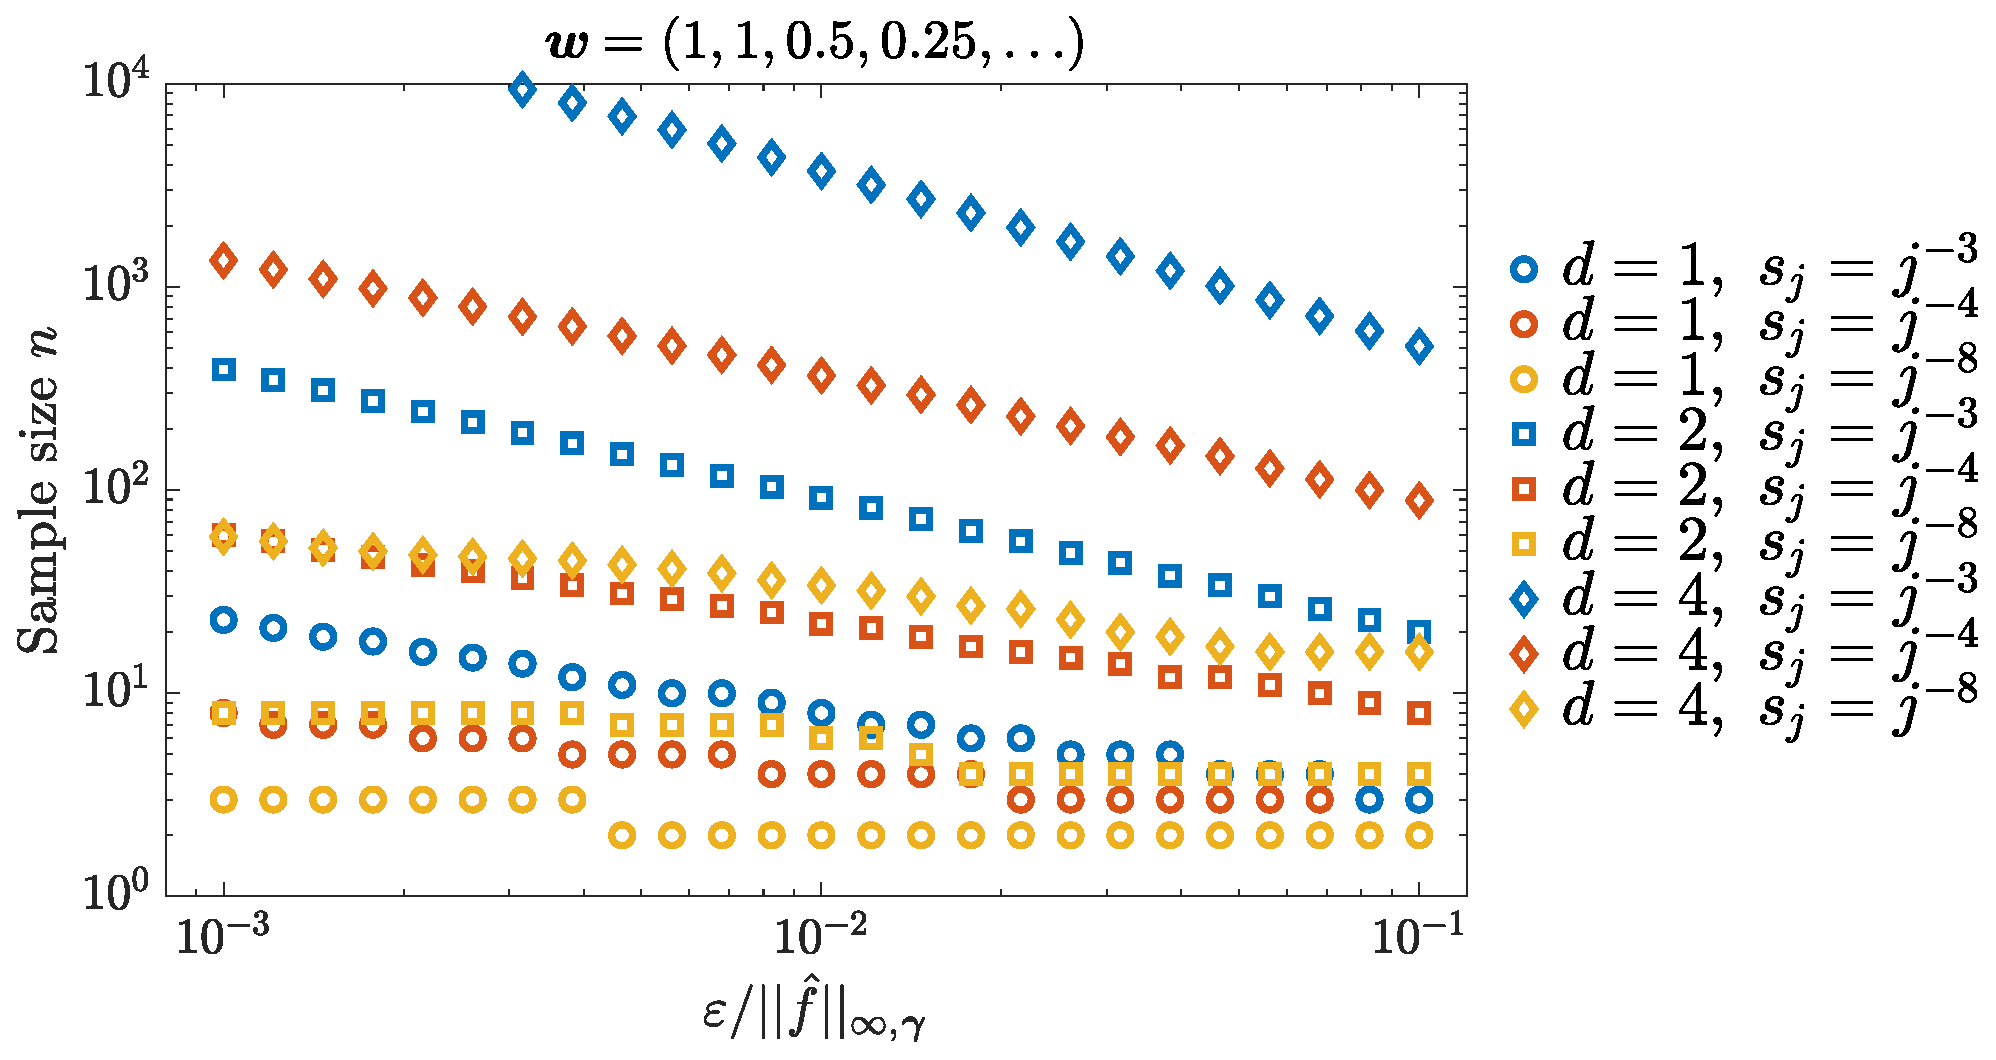
\includegraphics[width=0.95\textwidth]{FourierSampling/SampleSizeForDifferGamma.eps}}
\end{frame}


%\section{Inferred $\gamma$}

%\begin{frame}
%\frametitle{Algorithm When Both $\vgamma$ and $\bignorm[\infty,\vgamma]{\hf}$ Are Inferred}
%
%The order of sampling the series coefficients is determined by the $\vgamma$, but in practice the relative size of the series coefficients are not known, and thus $\vgamma$ should be inferred.  As a first step we try
%\begin{equation*}
%\gamma_{\vj} = \Gamma_{\norm[0]{\vj}} \prod_{\substack{\ell = 1 \\ j_\ell > 0}}^d w_{\ell} s_{j_\ell}, \qquad \Gamma_0  = s_1 = 1, \qquad 
%\begin{cases}
%w_\ell = \text{coordinate importance} \\
%\Gamma_r = \text{order size} \\
%s_j =  \text{smoothness degree}
%\end{cases}
%\end{equation*}
%with the $\Gamma_r$ and $s_j$ fixed, but the $w_\ell$ inferred.  \alert{We want to infer the relative importance of the different coordinates.}
%

%\end{frame}

\begin{frame}
\frametitle{Algorithm When Both $\vgamma$ and $\bignorm[\infty,\vgamma]{\hf}$ Are Inferred}

{\footnotesize
\begin{algorithmic}[1]
	
	\REQUIRE \begin{itemize}
		\item $\vGamma = $ vector of order sizes \qquad 
		\insertitemmarker $\vs = $ vector of smoothness degrees \qquad 
		\insertitemmarker $w^* = \max _k w_k$
		\item $n_0 = $ minimum number of wavenumbers in each coordinate \qquad 
		\insertitemmarker $C = $ inflation factor
		\item $\hf = $  a black-box series coefficient generator for the function of interest, $f$, where  $\bignorm[\infty,\vgamma]{\hf} \le C \bignorm[\infty,\vgamma]{\bigl(\hf_{\vj}\bigr)_{\vj \in \cj}}$, $\cj:= \{(0, \ldots, 0,j ,0 \ldots, 0) : j = 0, \ldots, n_0\}$ for all $\vgamma$
		\item $\varepsilon = $ positive absolute error tolerance
	\end{itemize}
	
	\ENSURE  $\norm[\infty]{f - \fappx} \le \varepsilon$
	
	\STATE Evaluate $\hf(\vj)$ for $\vj \in  \cj$
	
	\STATE Define $\vw = \min \argmin_{w_\ell \le w^*} \bignorm[\infty,\vgamma]{\bigl(\hf_{\vj}\bigr)_{\vj \in \cj}}$

	\STATE Let $n = \min \left\{ n' : \sum_{i = n'+1}^{\infty} \gamma_{\vj_i} \le \frac{\varepsilon}{C \bignorm[\infty,\vgamma]{\bigl(\hf_{\vj}\bigr)_{\vj \in \cj}}} \right \}$
	
	\STATE Compute $\fappx = \sum_{i=1}^n \hf(\vj_i) \phi_{\vj_i}$
	
\end{algorithmic}
}

\vspace{-3ex}

Computational cost is $\displaystyle n = \Order\left(\left[\varepsilon^{-1} C\bignorm[\infty,\vgamma]{\hf}   \alert{\bignorm[1/q]{\vgamma}}  \right]^{1/(q-1)} \right)$


\end{frame}

\begin{frame}
\frametitle{Example}

\vspace{-3ex}
$f$ manufactured in terms of random series coefficients

\vspace{-2ex}

\begin{tabular}{>{\centering}m{0.5\textwidth}>{\centering}m{0.48\textwidth}}
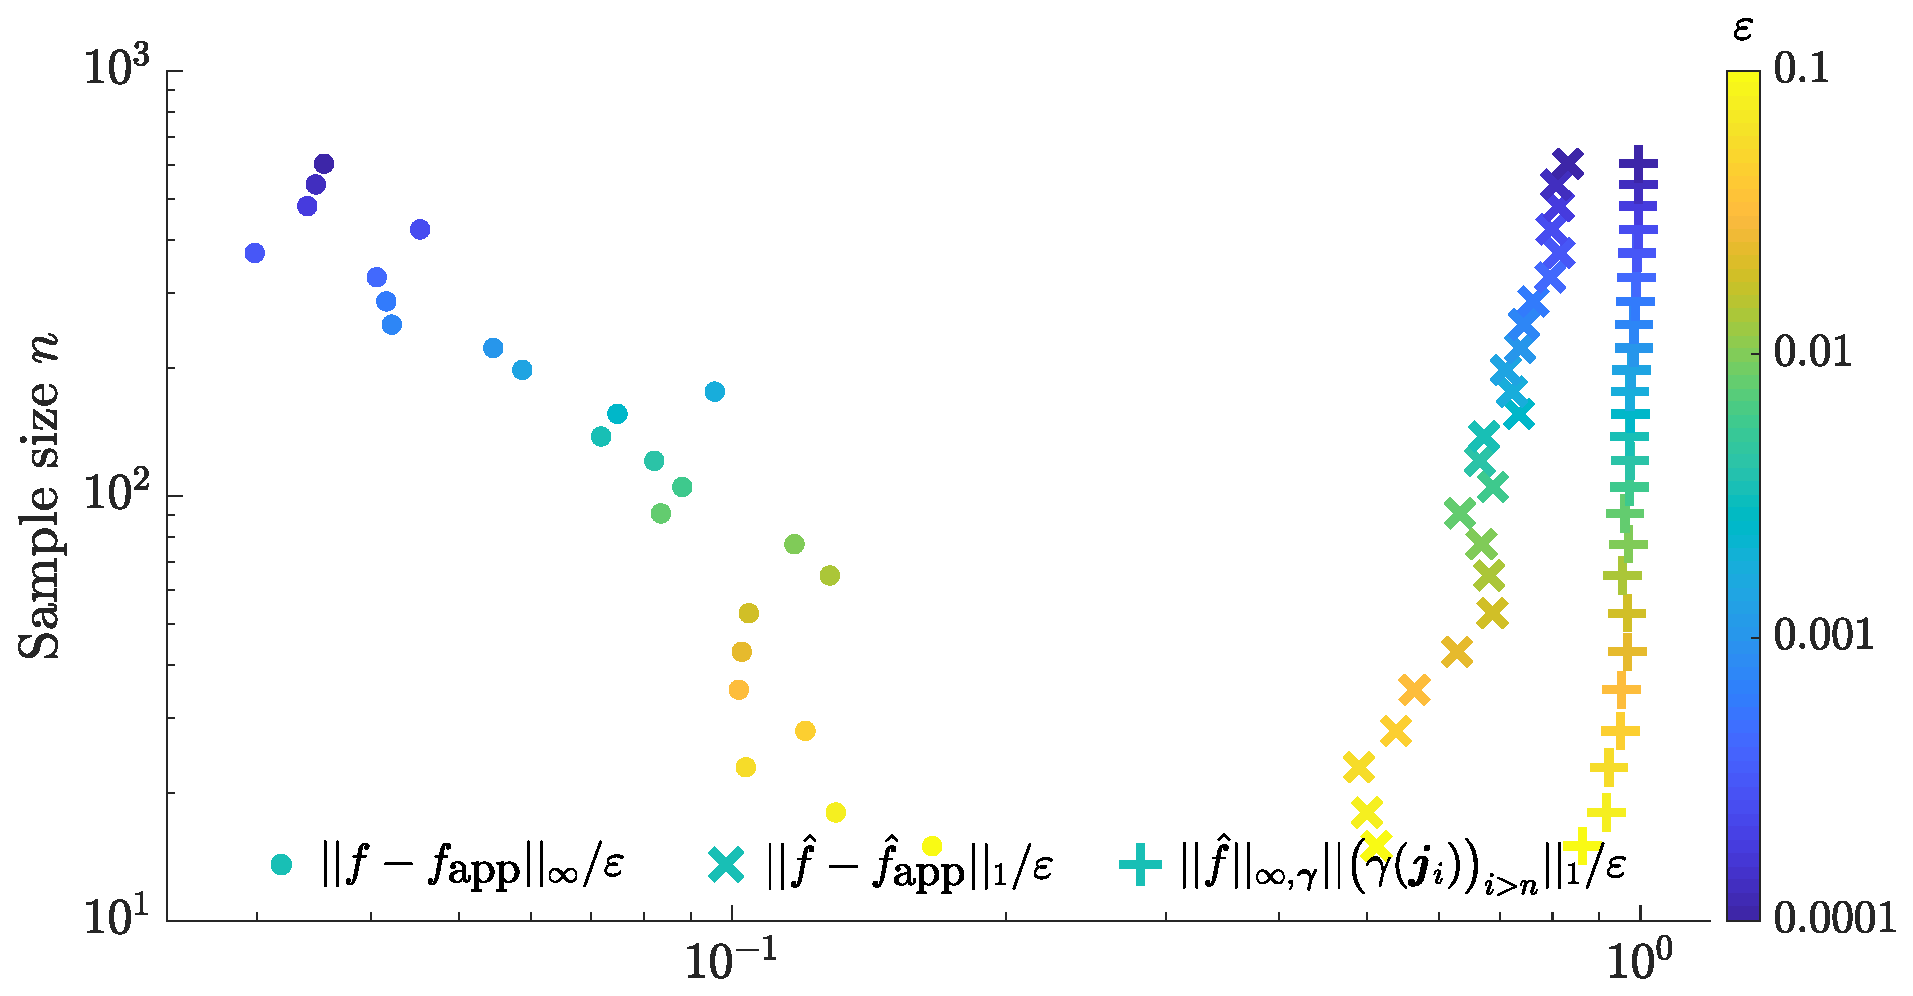
\includegraphics[width= 0.5\textwidth]{FourierSampling/SimDirectErr.eps} &
\includegraphics[width= 0.3\textwidth]{FourierSampling/SimDirectFun.eps} \newline
\includegraphics[width= 0.3\textwidth]{FourierSampling/SimDirectFunErr.eps}
\end{tabular}

\end{frame}


\section{Approx.\ by Function Values}

\begin{frame}
\frametitle{A Gap Between Theory and Practice}

\vspace{-3ex}

\begin{tabular}{>{\flushright}m{0.12\textwidth}>{\centering}m{0.7\textwidth}>{\flushleft}m{0.12\textwidth}}
Theory using series coefficients
& \includegraphics[width=0.7\textwidth]{ProgramsImages/ChinaBridgeGap.jpg}
\\
\hfill \hfill \scriptsize{ \href{http://www.chinadaily.com.cn/china/2014-05/13/content_17504637_5.htm}{Photo Credit: Xinhua}}
& Practice using function values
\end{tabular}
\end{frame}


\begin{frame}
\frametitle{A Very Sparse Grid on $[-1,1]^d$}
\vspace{-5ex}
\begin{equation*}
\begin{array}{r|cccccccc}
j & 0  & 1 & 2 & 3 & 4 & \cdots \tabularnewline
\text{van der Corput } t_j & 0 & 1/2 & 1/4 & 3/4 &  1/8 & \cdots \tabularnewline
\psi(t_j) :=  2(t_j + 1/3 \bmod 1)-1 & -1/3 & 2/3 & 1/6 & -5/6 & -1/12 & \cdots \tabularnewline
\psi(t_j) :=  -\cos(\pi(t_j + 1/3 \bmod 1)) & -0.5 & 0.8660 & 0.2588 & -0.9659 & -0.1305 & \cdots
\end{array}
\end{equation*}
To estimate $\hf(\vj)$, $\vj \in \cj$, use the design $\{(\psi(t_{j_1}), \ldots, \psi(t_{j_d}) : \vj \in \cj\}$.  E.g., for 
\[
\cj = \{(0,0,0,0), (1,0,0,0), (0,1,0,0), (0,0,1,0), (0,0,0,1), (2,0,0,0), (3,0,0,0), (1,1,0,0)\}
\]

\vspace{-4ex}

\begin{center}
	\begin{tabular}{>{\centering}m{0.25\linewidth}@{\qquad \qquad}>{\centering}m{0.25\linewidth}}
		Even Points& ArcCos Points \tabularnewline
		\includemedia[
		width=\linewidth,
		height=\linewidth,
		totalheight = \linewidth,
		activate=pageopen,
		passcontext,  %show VPlayer's right-click menu
		addresource=ProgramsImages/evenVerySparse.mp4,
		flashvars={
			%important: same path as in `addresource'
			source=ProgramsImages/evenVerySparse.mp4
		}
		]{$\cdot$}{VPlayer.swf}
		&
		\includemedia[
		width=\linewidth,
		height=\linewidth,
		totalheight = \linewidth,
		activate=pageopen,
		passcontext,  %show VPlayer's right-click menu
		addresource=ProgramsImages/acosVerySparse.mp4,
		flashvars={
			%important: same path as in `addresource'
			source=ProgramsImages/acosVerySparse.mp4
		}
		]{$\cdot$}{VPlayer.swf}
	\end{tabular}
\end{center}


\end{frame}

\begin{frame}
\frametitle{Algorithm Using Function Values When Both $\vgamma$ and $\bignorm[\infty,\vgamma]{\hf}$ Are Inferred}

{\footnotesize
	\begin{algorithmic}[1]
		
		\REQUIRE \begin{itemize}
			\item $\vGamma = $ vector of order sizes \qquad 
			\insertitemmarker $\vs = $ vector of smoothness degrees \qquad 
			\insertitemmarker $w^* = \max _k w_k$
			\item $n_0 = $ minimum number of wavenumbers in each coordinate \qquad 
			\insertitemmarker $C = $ inflation factor
			\item $f = $  a black-box function value generator \quad 
			\insertitemmarker $\varepsilon = $ positive absolute error tolerance
		\end{itemize}
		
		\ENSURE  $\norm[\infty]{f - \fappx} \le \varepsilon$
		
		\STATE Approximate $\hf(\vj)$ for $\vj \in  \cj:= \{(0, \ldots, 0,j ,0 \ldots, 0) : j = 1, \ldots, n_0\}$ by interpolating the function data $\{(\vx_\vj,f(\vx_\vj)) : \vx_\vj = \psi(t_{j_1}), \ldots, \psi(t_{j_d}), \  \vj \in \cj\}$
		
		\STATE Define $\vw = \min \argmin_{w_\ell \le w^*} \bignorm[\infty,\vgamma]{\bigl(\hf_{\vj}\bigr)_{\vj \in \cj}}$
		
		\WHILE {$C \bignorm[\infty,\vgamma]{\bigl(\hf_{\vj}\bigr)_{\vj \in \cj}} \sum_{\vj \notin \cj} \gamma_{\vj} > \varepsilon$}
		
		\STATE Add $\argmin_{\vj \notin \cj} \gamma_{\vj}$ to $\cj$
		
		\STATE Approximate $\hf(\vj)$ for $\vj \in  \cj$ by interpolating the function data $\{(\vx_\vj,f(\vx_\vj)) : \vx = \psi(t_{j_1}), \ldots, \psi(t_{j_d}), \  \vj \in \cj\}$
		
		\ENDWHILE
		
		\STATE Compute $\fappx = \sum_{\vj \in \cj} \hf(\vj) \phi_{\vj}$
		
	\end{algorithmic}
}

\end{frame}

\begin{frame}
\frametitle{Example\footfullcite{BinSur13}}

\vspace{-9ex}
\[
{} \qquad \qquad f(\vx) = \exp((x_2+1)(x_3+1)/4) \cos((x_2+1)/2 + (x_3+1)/2), \quad d = 6
\]
\vspace{-4ex}

\begin{tabular}{>{\centering}m{0.5\textwidth}>{\centering}m{0.48\textwidth}}
	\includegraphics[width= 0.5\textwidth]{FourierSampling/sim_eval_results_chsan10_ac1Err.eps} &
	\includegraphics[width= 0.3\textwidth]{FourierSampling/sim_eval_results_chsan10_ac1Fun.eps} \newline
	\includegraphics[width= 0.3\textwidth]{FourierSampling/sim_eval_results_chsan10_ac1FunErr.eps}
\end{tabular}



\end{frame}


\begin{frame}
\frametitle{OTL CircuitExample\footfullcite{BinSur13}}

\vspace{-6ex}

\begin{tabular}{>{\centering}m{0.5\textwidth}>{\centering}m{0.48\textwidth}}
	\includegraphics[width= 0.5\textwidth]{FourierSampling/sim_eval_results_otlcircuit_ac1Err.eps} &
	\includegraphics[width= 0.3\textwidth]{FourierSampling/sim_eval_results_otlcircuit_ac1Fun.eps} \newline
	\includegraphics[width= 0.3\textwidth]{FourierSampling/sim_eval_results_otlcircuit_ac1FunErr.eps}
\end{tabular}



\end{frame}



\begin{frame}
\frametitle{Summary}
\vspace{-3ex}
\begin{itemize}
	\item Functions must be \alert{nice} to succeed with few function values
	
	\item Ideas underlying \alert{experimental design} and \alert{tractability} show us how to define \alert{``nice''}
	
	\begin{itemize}
		\item Effect sparsity, hierarchy, heredity, and smoothness
		
		\item Product, order, and smoothness dependent (POSD) weighted function spaces
	\end{itemize}
	
	\item \alert{Infer} properties of $f$ from limited data ($\vgamma$, $\bignorm[\infty, \vgamma]{\hf}$, $\hf$)
	
	\item Must assume some structure on weights to make  progress at all
	
	\item \alert{Design} determined by wavenumbers included in approximation via van der Corput, preserves low condition number of the design matrix
	
	\item \alert{Gap} in theory when sampling function values versus series coefficients
	
	\item Sample size seems to be larger than necessary
	
	\item Can we also infer the smoothness weights?
	
\end{itemize}


\end{frame}


\finalthanksnote{These slides are  available at \\  \href{https://speakerdeck.com/fjhickernell/samsi-qmc-transition-2018-may}{\nolinkurl{speakerdeck.com/fjhickernell/samsi-qmc-transition-2018-may}}}

\thankyouframe

\printbibliography

\section{Appendix}

\begin{frame}[label = OptimalProof]
\frametitle{In What Sense Is This Optimal?}
\vspace{-7ex}
\begin{gather*}
f(\vx) = \sum_{\vj \in \natzero^d} \hf(\vj) \phi_{\vj}(\vx), \quad \hf(\vj) = \frac{\ip{f}{\phi_{\vj}}}{\ip{\phi_{\vj}}{\phi_{\vj}}}, 
 \quad \norm[\infty]{\phi_{\vj}}=1, \quad
\bignorm[q,\vgamma]{\hf} = \norm[q]{\left( \frac{\bigabs{\hf(\vj)}}{\gamma_{\vj}} \right)_{\vj \in \natzero^d}}
\\
\gamma_{\vj_1} \ge \gamma_{\vj_2} \ge \cdots, \quad
\fappx(\vx) = \sum_{i=1}^{n} \hf(\vj_i) \phi_{\vj_i}, \quad
\norm[\infty]{f - \fappx}
\overset{\text{loose}}{\le}  \bignorm[1]{\hf - \hfappx} \underset{\text{optimal}}{\overset{\text{tight}}{\le}} \bignorm[\infty,\vgamma]{\hf} \sum_{i = n+1}^{\infty}  \gamma_{\vj_{i}}
\end{gather*}
For \alert{any other} approximation, $g$, based on series coefficients, $\bigl\{\hf(\vj) \bigr\}_{\vj \in \cj}$ with $\abs{\cj} = n$,
\begin{align*}
\sup_{\substack{h\, : \,{\mathlarger \lVert} \hh {\mathlarger  \rVert}_{\infty,\vgamma} = {\mathlarger \lVert} \hf {\mathlarger  \rVert}_{\infty,\vgamma} \\ \hh(\vj) = \hf(\vj) \, \forall \vj \in \cj 
}} \bignorm[1]{\hh - \hg} 
&=  
\bignorm[1]{\bigl(\bigabs{\hf(\vj) -  \hg(\vj)} \bigr)_{\vj \in \cj}}
+
\sup_{h\, : \, 	{\mathlarger \lVert} \hh {\mathlarger  \rVert}_{\infty,\vgamma} = {\mathlarger \lVert} \hf {\mathlarger  \rVert}_{\infty,\vgamma} }  
\bignorm[1]{\bigl(\bigabs{\hh(\vj) -  \hg(\vj)} \bigr)_{\vj \notin \cj}}
\\
& 
\ge \sup_{h\, : \, 	{\mathlarger \lVert} \hh {\mathlarger  \rVert}_{\infty,\vgamma} = {\mathlarger \lVert} \hf {\mathlarger  \rVert}_{\infty,\vgamma} }  
\bignorm[1]{\bigl(\hh(\vj) \bigr)_{\vj \notin \cj}}
=  \sup_{h\, : \, 	{\mathlarger \lVert} \hh {\mathlarger  \rVert}_{\infty,\vgamma} = {\mathlarger \lVert} \hf {\mathlarger  \rVert}_{\infty,\vgamma} }  
\bignorm[\infty,\vgamma]{\hh} \sum_{\vj \notin \cj}  \gamma_{\vj} \\
&
\ge \bignorm[\infty,\vgamma]{\hf} \sum_{i = n+1}^{\infty}  \gamma_{\vj_{i}} \qquad \text{\beamerreturnbutton{\hyperlink{ApproxFourier}{back}}}
\end{align*}
\end{frame}

\begin{frame}
\frametitle{Inferring $\vgamma$ from Data}
Given (estimates of) series coefficients, $\hf(\vj)$ for $\vj \in \cj := \{(0, \ldots, 0,j ,0 \ldots, 0) : j = 1, \ldots, n_0\}$, and fixed $\{\Gamma_r\}_{r=0}^d$, and $\{s_j\}_{f=0}^{\infty}$, note that
\begin{equation*}
\bignorm[\infty,\vgamma]{\bigl(\hf(\vj)\bigr)_{\vj \in \cj} } =  \max_{\vj \in \cj} \frac{\normabs{\hf(\vj)}}{\gamma_{\vj}} =  \frac{1}{\Gamma_1 } \max_{k = 1, \ldots, d}   \frac{\hf_{k,\max}}{w_k}, \qquad  \hf_{k,\max} : = \sup_{j = 1, \ldots, n_0} \frac{\normabs{\hf(j\ve_k)}}{s_j}
\end{equation*}
We choose
\begin{equation*}
w_k =    \frac{\hf_{k,\max}}{\displaystyle \max_\ell \hf_{\ell,\max}}, \qquad \bignorm[\infty,\vgamma]{\bigl(\hf(\vj)\bigr)_{\vj \in \cj} } = \frac{\displaystyle \max_\ell \hf_{\ell,\max}}{\Gamma_1}
\end{equation*}

\end{frame}

\begin{frame}
\frametitle{Tail Sum of $\vgamma$}
\vspace{0ex}
The term 
\begin{equation*}
\sum_{i = n+1}^{\infty}  \gamma_{\vj_{i}} = \sum_{i = 1}^{\infty}  \gamma_{\vj_{i}} - \sum_{i =1}^{n}  \gamma_{\vj_{i}}
\end{equation*}
appears in the error bound.  For certain $\vgamma$ of PSD form, we can compute the first sum on the right:
\begin{equation*}
\sum_{\vj \in \natzero^d} \gamma_{\vj} = \sum_{\fu \subseteq 1:d} \left[ \left(\prod_{\ell \in \fu} w_{\ell} \right) \left(\sum_{j=1}^{\infty} s_{j} \right)^{\abs{\fu}} \right]  = \prod_{\ell = 1}^d ( 1 + w_{\ell}  s_{\text{sum}} ), \qquad s_{\text{sum}} = \sum_{j=1}^{\infty} s_{j}
\end{equation*}


\end{frame}





\end{document}


\begin{frame}
\frametitle{Algorithm When Both $\vgamma$ and $\bignorm[\infty,\vgamma]{\hf}$ Are Known}

\begin{algorithmic}[1]
	
	\REQUIRE 	\begin{itemize}
		\item $\vgamma = $ vector of weights with ordering $\gamma_{\vj_1} \ge \gamma_{\vj_2} \ge \cdots$
		\item $\hf = $  black-box series coefficient generator
		\item $\bignorm[\infty,\vgamma]{\hf} = $ norm of the series coefficients
		\item $\varepsilon = $ positive absolute error tolerance
	\end{itemize}
	
	\ENSURE  $\norm[\infty]{f - \fappx} \le \varepsilon$
	
	\STATE Let $n = \min \left\{ n' : \sum_{i = n'+1}^{\infty} \gamma_{\vj_i} \le \frac{\varepsilon}{\bignorm[\infty,\vgamma]{\hf}} \right \}$
	
	\STATE Compute $\fappx = \sum_{i=1}^n \hf(\vj_i) \phi_{\vj_i}$
	
\end{algorithmic}

\vspace{-3ex}

Computational cost is $\displaystyle n = \Order\left(\left[\varepsilon^{-1} \bignorm[\infty,\vgamma]{\hf}   \alert{\bignorm[1/q]{\vgamma}}  \right]^{1/(q-1)} \right)$; $\vgamma$ determines the \alert{design}

\end{frame}

\begin{frame}
\frametitle{Algorithm When $\vgamma$ Is Known and $\bignorm[\infty,\vgamma]{\hf}$ Is Inferred}

\begin{algorithmic}[1]

\REQUIRE 	\begin{itemize}
	\item $\vgamma = $ vector of weights with ordering $\gamma_{\vj_1} \ge \gamma_{\vj_2} \ge \cdots$
	\item $n_0 = $ minimum number of wavenumbers \qquad \qquad 
	\insertitemmarker $C = $ inflation factor
	\item $\hf = $ black-box series coefficient generator for the function of interest, $f$, where  $\bignorm[\infty,\vgamma]{\hf} \le C \bignorm[\infty,\vgamma]{\bigl(\hf_{\vj_i}\bigr)_{i=1}^{n_0}}$
	\item $\varepsilon = $ positive absolute error tolerance
\end{itemize}

\ENSURE  $\norm[\infty]{f - \fappx} \le \varepsilon$

\STATE Evaluate $\hf(\vj_1), \ldots, \hf(\vj_{n_0})$

\STATE Let $n = \min \left\{ n' > n_0 : \sum_{i = n'+1}^{\infty} \gamma_{\vj_i} \le \frac{\varepsilon}{C \bignorm[\infty,\vgamma]{\bigl(\hf_{\vj_i}\bigr)_{i=1}^{n_0}}} \right \}$

\STATE Compute $\fappx = \sum_{i=1}^n \hf(\vj_i) \phi_{\vj_i}$

\end{algorithmic}

\vspace{-3ex}

Computational cost is $\displaystyle n = \Order\left(\left[\varepsilon^{-1} C\bignorm[\infty,\vgamma]{\hf}   \alert{\bignorm[1/q]{\vgamma}}  \right]^{1/(q-1)} \right)$; $\vgamma$ determines the \alert{design}


\end{frame}





